\section{Ansätze Office  vs  \LaTeX}
% \begin{frame}
 	\frametitle{Inhalt}
 	\tableofcontents[%
 		currentsection, % causes all sections but the current to be shown in a semi-transparent way.
% % 		currentsubsection, % causes all subsections but the current subsection in the current section to ...
% % 		hideallsubsections, % causes all subsections to be hidden.
% 		hideothersubsections, % causes the subsections of sections other than the current one to be hidden.
% % 		part=, % part number causes the table of contents of part part number to be shown
% 		pausesections, % causes a \pause command to be issued before each section. This is useful if you
% 		pausesubsections, %  causes a \pause command to be issued before each subsection.
% % 		sections={ overlay specification },
 	]
 \end{frame}
\begin{frame}{Ansätze Office  vs  \LaTeX}
	\begin{columns}
	
		 \column{0.45\textwidth}
		Office
		\begin{itemize}
			\item WYSIWYG
			\item volle Kontrolle des Nutzers über die Formatierung
			\item Anwender MUSS sich um alles selbst kümmern
			\item Arbeitsaufwand bleibt immer gleich
		\end{itemize}
		
		\column{0.45\textwidth}
		\LaTeX{}
		\begin{itemize}
				\item kein WYSIWYG
				\item Nutzer gibt absichtlich einen teil der Kontrolle ab
				\item Anwender kümmert sich nur um Format vorgaben
				\item Arbeitsaufwand sinkt, Autor kann sich auf das reine Schreiben konzentrieren
		\end{itemize}
	\end{columns}
\end{frame}
\begin{frame}{Arbeitsaufwand}
	\begin{figure}[htbp]
	\centering
		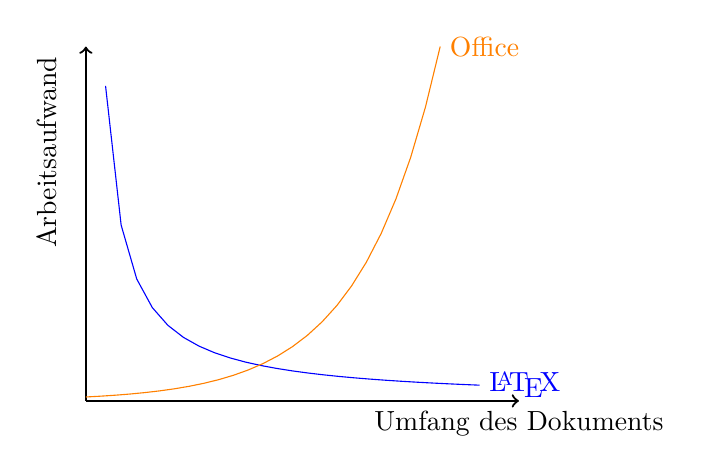
\begin{tikzpicture}[domain=0:5]
		
		  \draw[->,thick] (0,0)-- coordinate(x axis mid) (5.5,0) node[below] {Umfang des Dokuments };
		  \draw[->,thick] (0,0) -- coordinate(y axis mid) (0,4.5) node[left=0.5cm, rotate=90] {Arbeitsaufwand};
		  \draw[color=blue,domain=0.25:5] plot (\x,{ 1/ \x }) node[right] {\LaTeX};
		
		  \draw[color=orange,domain=0:4.5] plot (\x,{0.05*exp(\x)}) node[right] {Office};
		\end{tikzpicture}
	\end{figure}
\end{frame}
\begin{frame}{Wann nehme ich was?}
	\begin{columns}
	\centering
		\begin{column}{0.45\textwidth}
			Office
			\begin{itemize}[<+->]
			\item kleiner arbeiten 2-3
			\item Effektvolle Präsentationen
			\item wenn es schnell gehen muss und der Umfang gering ist
			\end{itemize}
		\end{column}
		\begin{column}{0.45\textwidth}
			\LaTeX
			\begin{itemize}[<+->]
			\item größere Arbeiten (Bachelor-,Master-,Diplomarbeit, Bücher)
			\item wenn mehrere Autoren beteiligt sind
			\item wenn ein Dokument Jahre später immer noch gleich aussehen soll
			\end{itemize}
		\end{column}
	\end{columns}
\end{frame}